\chapter{Introduction}
In 1971, the first email was sent\cite{tomlinson2009first}.
Email is implemented using decentralized protocols for sending simple messages between recipients, specified for example in the \ac{SMTP} \ac{RFC}\cite{RFC5321}.
One may register with an email provider, and write messages to any other provider implementing the same protocols, as long as they have the recipient's address, known as an email address.
Mobile providers similarly allow people to contact others outside of their network.
This is an elegant, scalable and privacy-respecting architecture.
However, there's been a growing trend of \textit{walled gardens}\cite{walled_gardens_gunnar_wolf_acm_2018}, where users may only contact other users of the same service.
Examples of such services are Slack\cite{walled_gardens_gunnar_wolf_acm_2018}; WhatsApp, which has announced that its userbase has now exceeded two billion users\cite{whatsapp_2b_users_archive_org}; and Facebook Messenger, which similarly reported having 1.3 billion users\cite{messenger_1pt3b_users}.

\section{Initial Problem}\label{subsec:initial_problem_statement}
\paragraph{Walled Gardens}
Closed-platform services, or walled gardens, are a fragmenting influence on peoples' communication.
Although these services run over the internet, they are designed in isolation, and do not adhere to an external standard.
In order to use such a service, a user must acquire a client designed for this private procotol.
This has the negative effect of people having to keep track of whom to contact on which service.
They are forced to rely on external vendors for the storage and security of their messages.
We refer to this problem as \textit{the walled garden problem}.

\paragraph{Security}
In the typical client-server architecture, the client is forced to operate with some level of trust.
In the case of email, the original architecture required that both participants be online, but has now adapted such that some server just needs to receive it and be able to pass it on to the recipient when possible\cite{tomlinson2009first}.
Platforms which follow this architecture for messaging therefore store the messages of all participants.
The storage format and security depends on the software run on the server, which receives, stores and passes the messages on.
For closed-source vendors, it is intractable to know whether the messages passed are done so securely, or whether third parties can access the data.
Users are therefore forced to either rely on the word of the service providers, or use an alternative.
In the cases of WhatsApp and Facebook Messenger, several such features are advertised, but regardless not verified\cite{twitter_comms_protocol_comparison}.

\section{Matrix}
The Matrix standard is a potential solution to the \textit{walled garden problem}, and is described as an "open standard for interoperable, decentralised, real-time communication over IP"\cite{matrix_org}.
On the choice of the name Matrix, the Matrix organization states: "We are called Matrix because we provide a structure in which all communication can be matrixed together."\cite{matrix_org_faq}

\begin{figure}[h]
    \centering
    Matrix = \bordermatrix{~      & Work & Friends & Family & Hobbies\cr
                        Msg       & 1 & 1 & 1 & 1\cr
                        Voice     & 1 & 1 & 1 & 1\cr
                        Video     & 1 & 1 & 1 & 1\cr
                        Bots      & 1 & 1 & 1 & 1\cr
                        Bridges   & 1 & 1 & 1 & 1\cr}
    \caption{Matrix provides the fundamental structure for matrixing together all communication.}
    \label{}
\end{figure}

The Matrix open standard\cite{matrix_org_spec} is a specification for a network of independent servers which may communicate.
It supports more recent features, such as live messaging, calls, and video conferencing.
Figure \ref{fig:matrix_structure} demonstrates how four users might be connected via the Matrix protocol.
There are three servers: matrix.a.com, matrix.b.com, and a Third Party, e.g. Slack.
The users are @a:a.com, @b:b.com, c, and @d:b.com.
The third party protocol is enabled via a Bridge to matrix.a.com, which allows the native Matrix users to communicate with c, and vice versa.

\begin{figure}[h]
    % Graphic for TeX using PGF
% Title: /home/lihram/git/github.com/lihram/p8-matrix-p2p/report/graphics/matrix.dia
% Creator: Dia v0.97.3
% CreationDate: Thu Apr  2 21:27:29 2020
% For: lihram
% \usepackage{tikz}
% The following commands are not supported in PSTricks at present
% We define them conditionally, so when they are implemented,
% this pgf file will use them.
\ifx\du\undefined
  \newlength{\du}
\fi
\setlength{\du}{15\unitlength}
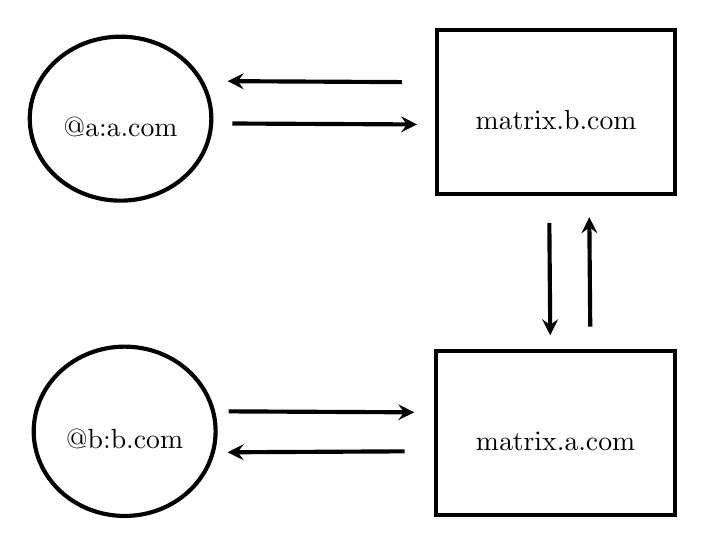
\begin{tikzpicture}
\pgftransformxscale{1.000000}
\pgftransformyscale{-1.000000}
\definecolor{dialinecolor}{rgb}{0.000000, 0.000000, 0.000000}
\pgfsetstrokecolor{dialinecolor}
\definecolor{dialinecolor}{rgb}{1.000000, 1.000000, 1.000000}
\pgfsetfillcolor{dialinecolor}
\definecolor{dialinecolor}{rgb}{1.000000, 1.000000, 1.000000}
\pgfsetfillcolor{dialinecolor}
\pgfpathellipse{\pgfpoint{23.159091\du}{11.454516\du}}{\pgfpoint{2.187187\du}{0\du}}{\pgfpoint{0\du}{1.975319\du}}
\pgfusepath{fill}
\pgfsetlinewidth{0.100000\du}
\pgfsetdash{}{0pt}
\pgfsetdash{}{0pt}
\pgfsetmiterjoin
\definecolor{dialinecolor}{rgb}{0.000000, 0.000000, 0.000000}
\pgfsetstrokecolor{dialinecolor}
\pgfpathellipse{\pgfpoint{23.159091\du}{11.454516\du}}{\pgfpoint{2.187187\du}{0\du}}{\pgfpoint{0\du}{1.975319\du}}
\pgfusepath{stroke}
% setfont left to latex
\definecolor{dialinecolor}{rgb}{0.000000, 0.000000, 0.000000}
\pgfsetstrokecolor{dialinecolor}
\node at (23.159091\du,11.648578\du){@a:a.com};
\definecolor{dialinecolor}{rgb}{1.000000, 1.000000, 1.000000}
\pgfsetfillcolor{dialinecolor}
\pgfpathellipse{\pgfpoint{23.257966\du}{18.985725\du}}{\pgfpoint{2.191191\du}{0\du}}{\pgfpoint{0\du}{2.039375\du}}
\pgfusepath{fill}
\pgfsetlinewidth{0.100000\du}
\pgfsetdash{}{0pt}
\pgfsetdash{}{0pt}
\pgfsetmiterjoin
\definecolor{dialinecolor}{rgb}{0.000000, 0.000000, 0.000000}
\pgfsetstrokecolor{dialinecolor}
\pgfpathellipse{\pgfpoint{23.257966\du}{18.985725\du}}{\pgfpoint{2.191191\du}{0\du}}{\pgfpoint{0\du}{2.039375\du}}
\pgfusepath{stroke}
% setfont left to latex
\definecolor{dialinecolor}{rgb}{0.000000, 0.000000, 0.000000}
\pgfsetstrokecolor{dialinecolor}
\node at (23.257966\du,19.179788\du){@b:b.com};
\definecolor{dialinecolor}{rgb}{1.000000, 1.000000, 1.000000}
\pgfsetfillcolor{dialinecolor}
\fill (30.775500\du,9.312650\du)--(30.775500\du,13.262650\du)--(36.525500\du,13.262650\du)--(36.525500\du,9.312650\du)--cycle;
\pgfsetlinewidth{0.100000\du}
\pgfsetdash{}{0pt}
\pgfsetdash{}{0pt}
\pgfsetmiterjoin
\definecolor{dialinecolor}{rgb}{0.000000, 0.000000, 0.000000}
\pgfsetstrokecolor{dialinecolor}
\draw (30.775500\du,9.312650\du)--(30.775500\du,13.262650\du)--(36.525500\du,13.262650\du)--(36.525500\du,9.312650\du)--cycle;
% setfont left to latex
\definecolor{dialinecolor}{rgb}{0.000000, 0.000000, 0.000000}
\pgfsetstrokecolor{dialinecolor}
\node at (33.650500\du,11.481703\du){matrix.b.com};
\definecolor{dialinecolor}{rgb}{1.000000, 1.000000, 1.000000}
\pgfsetfillcolor{dialinecolor}
\fill (30.763900\du,17.046800\du)--(30.763900\du,20.996800\du)--(36.513900\du,20.996800\du)--(36.513900\du,17.046800\du)--cycle;
\pgfsetlinewidth{0.100000\du}
\pgfsetdash{}{0pt}
\pgfsetdash{}{0pt}
\pgfsetmiterjoin
\definecolor{dialinecolor}{rgb}{0.000000, 0.000000, 0.000000}
\pgfsetstrokecolor{dialinecolor}
\draw (30.763900\du,17.046800\du)--(30.763900\du,20.996800\du)--(36.513900\du,20.996800\du)--(36.513900\du,17.046800\du)--cycle;
% setfont left to latex
\definecolor{dialinecolor}{rgb}{0.000000, 0.000000, 0.000000}
\pgfsetstrokecolor{dialinecolor}
\node at (33.638900\du,19.215853\du){matrix.a.com};
\pgfsetlinewidth{0.100000\du}
\pgfsetdash{}{0pt}
\pgfsetdash{}{0pt}
\pgfsetbuttcap
{
\definecolor{dialinecolor}{rgb}{0.000000, 0.000000, 0.000000}
\pgfsetfillcolor{dialinecolor}
% was here!!!
\pgfsetarrowsend{stealth}
\definecolor{dialinecolor}{rgb}{0.000000, 0.000000, 0.000000}
\pgfsetstrokecolor{dialinecolor}
\draw (25.854118\du,11.570902\du)--(30.301569\du,11.593827\du);
}
\pgfsetlinewidth{0.100000\du}
\pgfsetdash{}{0pt}
\pgfsetdash{}{0pt}
\pgfsetbuttcap
{
\definecolor{dialinecolor}{rgb}{0.000000, 0.000000, 0.000000}
\pgfsetfillcolor{dialinecolor}
% was here!!!
\pgfsetarrowsend{stealth}
\definecolor{dialinecolor}{rgb}{0.000000, 0.000000, 0.000000}
\pgfsetstrokecolor{dialinecolor}
\draw (33.488145\du,13.966565\du)--(33.511070\du,16.671716\du);
}
\pgfsetlinewidth{0.100000\du}
\pgfsetdash{}{0pt}
\pgfsetdash{}{0pt}
\pgfsetbuttcap
{
\definecolor{dialinecolor}{rgb}{0.000000, 0.000000, 0.000000}
\pgfsetfillcolor{dialinecolor}
% was here!!!
\pgfsetarrowsend{stealth}
\definecolor{dialinecolor}{rgb}{0.000000, 0.000000, 0.000000}
\pgfsetstrokecolor{dialinecolor}
\draw (30.003544\du,19.468567\du)--(25.739493\du,19.491492\du);
}
\pgfsetlinewidth{0.100000\du}
\pgfsetdash{}{0pt}
\pgfsetdash{}{0pt}
\pgfsetbuttcap
{
\definecolor{dialinecolor}{rgb}{0.000000, 0.000000, 0.000000}
\pgfsetfillcolor{dialinecolor}
% was here!!!
\pgfsetarrowsend{stealth}
\definecolor{dialinecolor}{rgb}{0.000000, 0.000000, 0.000000}
\pgfsetstrokecolor{dialinecolor}
\draw (25.762418\du,18.505716\du)--(30.232794\du,18.528641\du);
}
\pgfsetlinewidth{0.100000\du}
\pgfsetdash{}{0pt}
\pgfsetdash{}{0pt}
\pgfsetbuttcap
{
\definecolor{dialinecolor}{rgb}{0.000000, 0.000000, 0.000000}
\pgfsetfillcolor{dialinecolor}
% was here!!!
\pgfsetarrowsend{stealth}
\definecolor{dialinecolor}{rgb}{0.000000, 0.000000, 0.000000}
\pgfsetstrokecolor{dialinecolor}
\draw (34.473920\du,16.465391\du)--(34.450995\du,13.829015\du);
}
\pgfsetlinewidth{0.100000\du}
\pgfsetdash{}{0pt}
\pgfsetdash{}{0pt}
\pgfsetbuttcap
{
\definecolor{dialinecolor}{rgb}{0.000000, 0.000000, 0.000000}
\pgfsetfillcolor{dialinecolor}
% was here!!!
\pgfsetarrowsend{stealth}
\definecolor{dialinecolor}{rgb}{0.000000, 0.000000, 0.000000}
\pgfsetstrokecolor{dialinecolor}
\draw (29.934769\du,10.573665\du)--(25.739493\du,10.550740\du);
}
\end{tikzpicture}

    \caption{Matrix allows users to communicate across servers. Using bridges, Matrix users may even communicate with people registered with third party protocols.}
    \label{fig:matrix_structure}
\end{figure}

The standard has been implemented by several clients\cite{matrix_org_clients}.
There is ongoing work on implementing SDKs\cite{matrix_org_sdks}, which provide the foundational logic for implementing more applications.
Through bridges, Matrix allows communicating with different protocols\cite{matrix_org_bridges}, such as WhatsApp or Messenger.
The reference implementation of the Matrix open standard is Synapse\cite{matrix_org_synapse}, which is written in Python.
The standard was declared stable and released as 1.0 on June 10th, 2019\cite{matrix_org_spec}, and is still very young.
Its limitations become apparent as one considers its applications, such as peer-to-peer Matrix.


\paragraph{Peer-to-Peer Matrix}
The Matrix team is working on Dendrite\cite{matrix_org_dendrite}, an experimental server written in Golang, which is the base for peer-to-peer experiments.
This approach overcomes some of the drawbacks of the classical implementation of Matrix, which requires each user to be registered with a homeserver with a DNS entry and a static IP address.
The development of Peer-to-Peer Matrix is currently experimental and ongoing.
Its application is currently limited to the web at \url{https://p2p.riot.im}, but could expand into other fields such as embedded, or mobile devices.

\paragraph{Smartphones}
Due to the popularity and widespread use of mobile phones, experimentation with peer-to-peer Matrix on smartphones would be an interesting task.
\textit{Besides an experimental browser-based solution\cite{fosdem_event_p2p_matrix}, there is no peer-to-peer Matrix application for mobile clients, such as smartphones.}

The benefits of having an on-device homeserver for a telephone would have strong benefits for users, such as:
\begin{itemize}
    \item Full control of data,
    \item No registration necessary, and
    \item Increased privacy.
\end{itemize}

\noindent Mobile devices are by definition constrained by battery life, and often a reduced form factor.
In order for peer-to-peer Matrix to succeed on mobile, it needs to respect the limited resources available on the device.


\begin{center}
    We propose the following initial problem: \textit{What can we do to get peer-to-peer Matrix on the smartphone, while respecting the constraints of mobile phones, such as battery life and memory usage?}
\end{center}

